C++ provides a framework for notification and handling of errors through its exception mechanism. Heterogeneous programming requires an additional level of error management beyond this, because some errors occur on a device or when trying to launch work on a device. These errors are typically decoupled in time from the host program’s execution, and as such they don’t integrate cleanly with classic C++ exception handling mechanisms. To solve this, there are additional mechanisms to make asynchronous errors as manageable and controllable as regular C++ exceptions.\par

Figure 5-1 shows two components of a typical application: (1) the host code that runs sequentially and submits work to the task graph for future execution and (2) the task graph which runs asynchronously from the host program and executes kernels or other actions on devices when the necessary dependences are met. The example shows a parallel\_for as the operation that executes asynchronously as part of the task graph, but other operations are possible as well as discussed in Chapters 3, 4, and 8.\par

\hspace*{\fill} \par %插入空行
Figure 5-1. Separation of host program and task graph executions
\begin{center}
	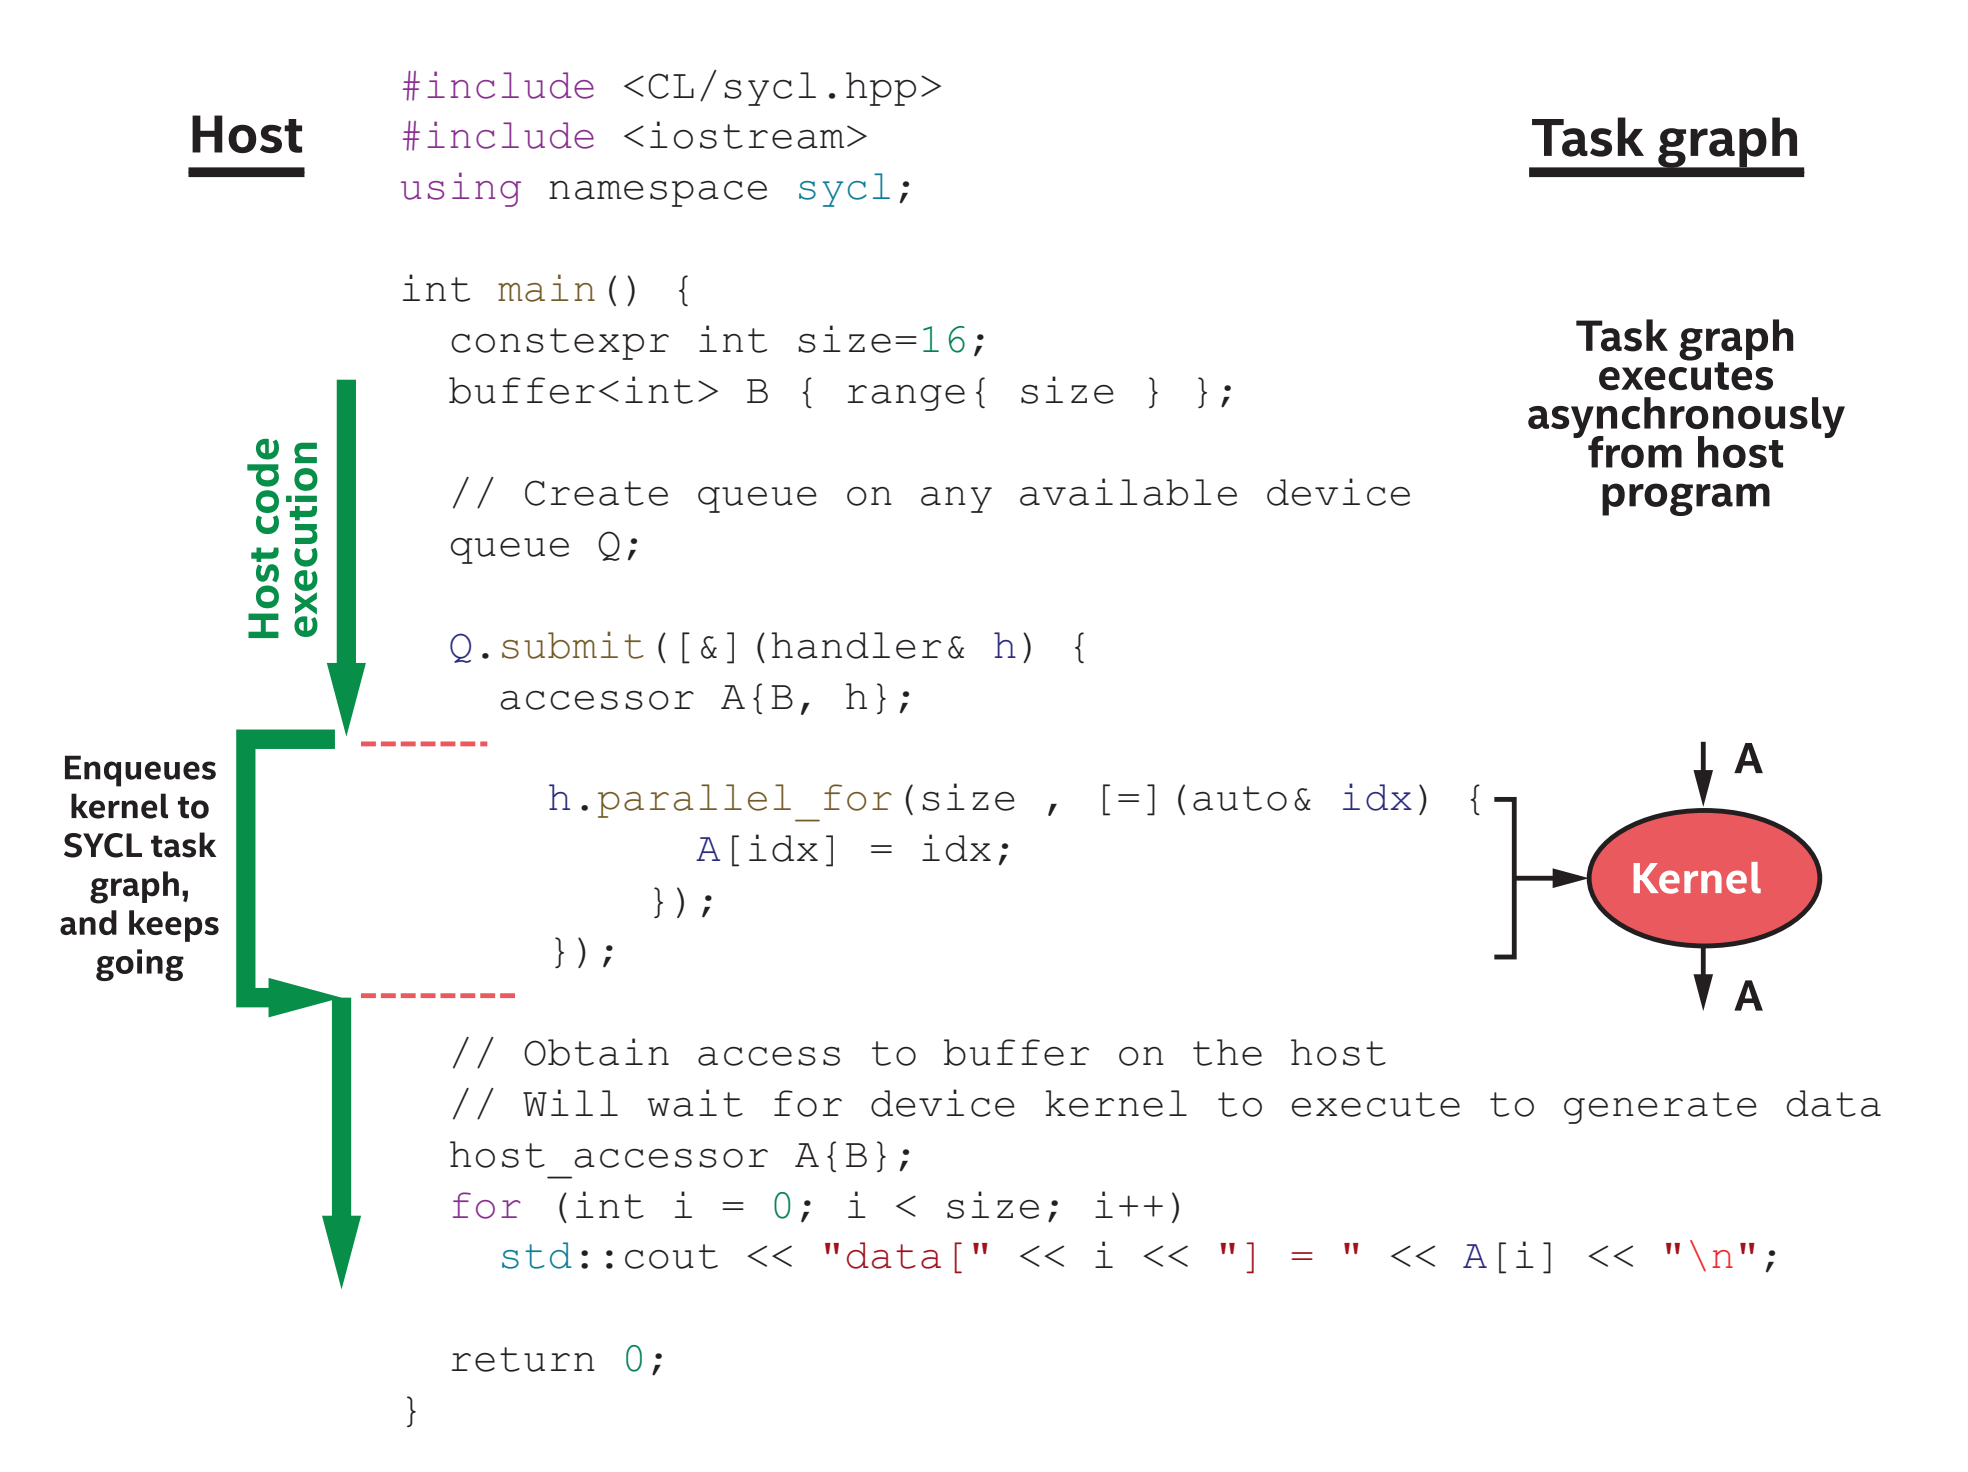
\includegraphics[width=1.0\textwidth]{content/chapter-5/images/2}
\end{center}

The distinction between the left and right (host and task graph) sides of Figure 5-1 is the key to understanding the differences between synchronous and asynchronous errors.\par

Synchronous errors occur when an error condition can be detected as the host program executes an operation, such as an API call or object constructor. They can be detected before an instruction on the left side of the figure completes, and the error can be thrown by the operation that caused the error immediately. We can wrap specific instructions on the left side of the diagram with a try-catch construct, expecting that errors occurring as a result of operations within the try will be detected before the try block ends (and therefore caught). The C++ exception mechanism is designed to handle exactly these types of errors.\par

Alternatively, asynchronous errors occur as part of the right side of Figure 5-1, where an error is only detected when an operation in the task graph is executed. By the time that an asynchronous error is detected as part of task graph execution, the host program has typically already moved on with its execution, so there is no code to wrap with a trycatch construct to catch these errors. There is instead an asynchronous exception handling framework to handle these errors that occur at seemingly random times relative to host program execution.\par










